\section{Ergebnisse}

\subsection{Zahlen ohne Optimierung}
Beim ersten Zoom ist ein 16-facher Zoom nicht mehr möglich, da die Matrix so gross wird, dass der Computer nicht genügend RAM freiräumen kann. Ausserdem dauert es dann schnell mal lange Zeit, einen 12-fachen Zoom mit der Auflösung 4'001 auf 2'667 Pixel zum Punkt -1.25 und mit 150 Iterationen etwa 45.6 Stunden zu berechnen.\\
Durch die CUDA-Optimierung kann man nur noch einen 6.25-fachen Zoom machen, dies liegt daran, dass die GPU nur noch 8GB VRAM und der PC 16GB RAM haben. Bei gleicher Einstellung, bis auf die Zoomtiefe von 6.25, konnte das Programm innerhalb von 2 Minuten und 34 Sekunden fertig rechnen. Dass ein Zoom nicht gleich tief möglich ist, ist eigentlich irrelevant, denn es geht ja darum, die Rechenleistung zu verringern und einen allfälligen Algorithmus zu finden. Mit demselben Programm sowie einem 1-fachen Zoom, dauert die Berechnung nun nur noch 49 Sekunden statt drei Stunden.
\subsection{Analyse der Ergebnisse}
\begin{figure}[!h]
	\centering
	\subfloat[1. Quadrant]{\scalebox{1}[-1]{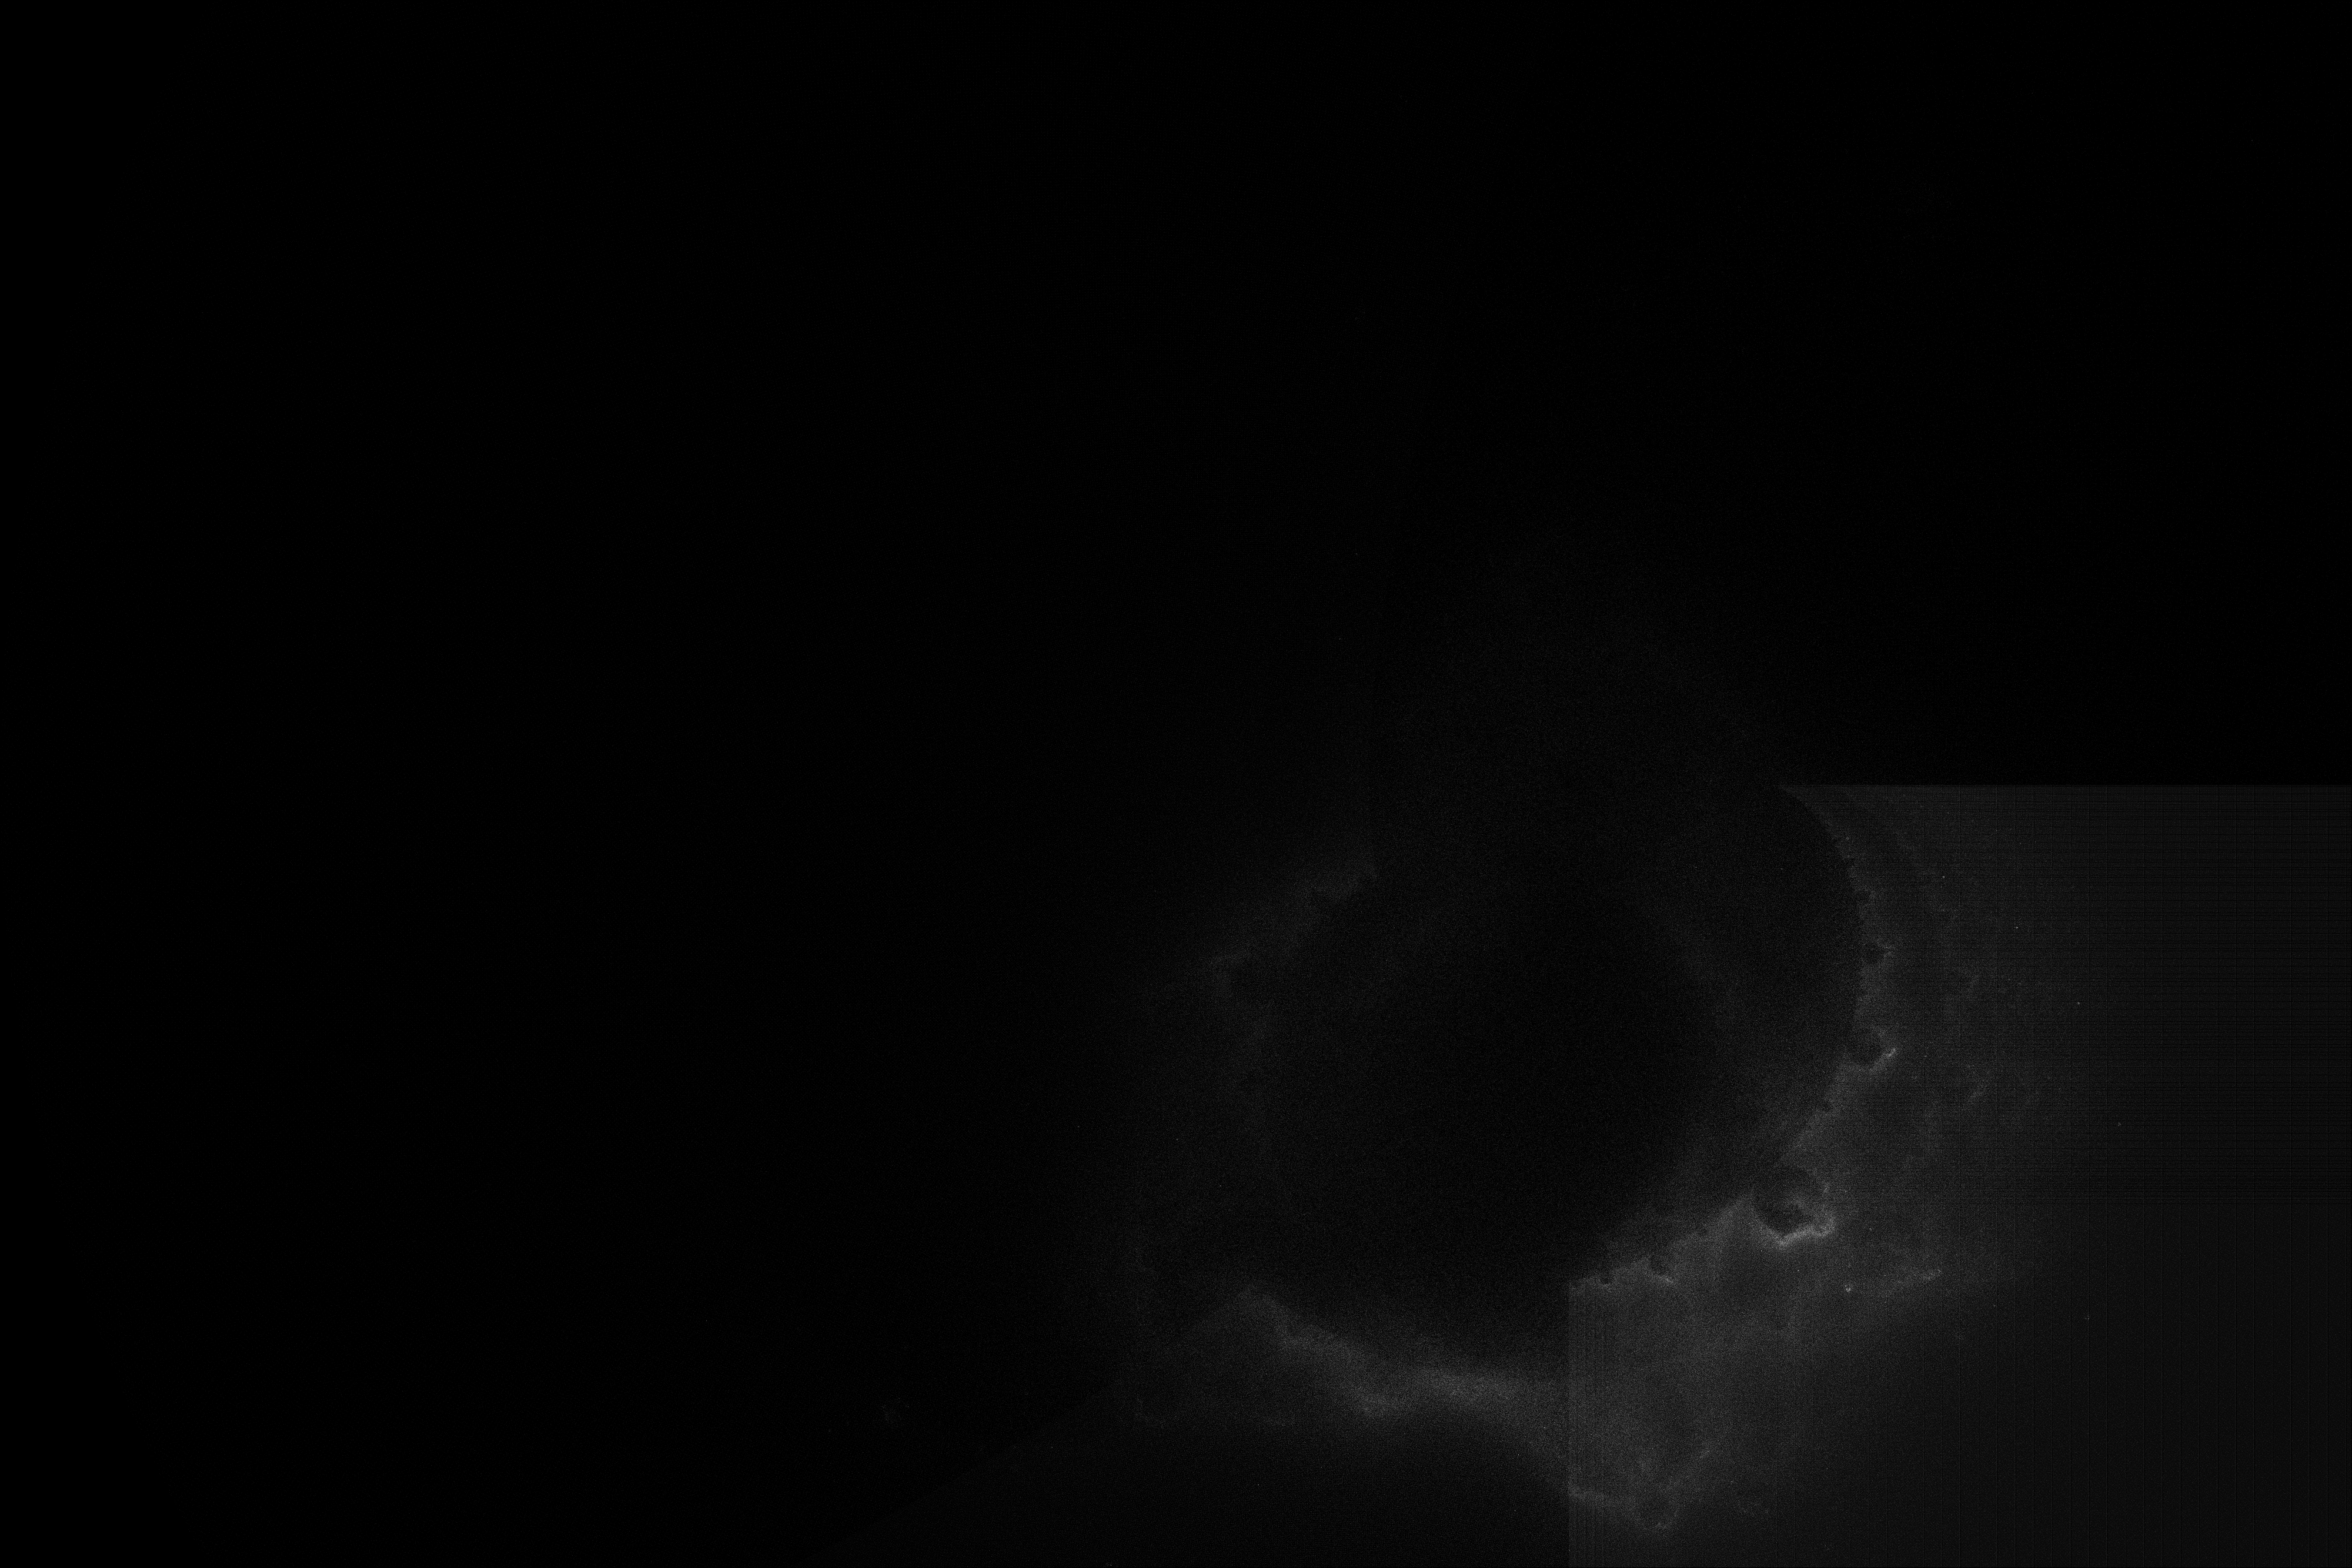
\includegraphics[width=.49\textwidth]{Pictures/1AnalyBuddhabrotmengeWithZoomGPU1ToPoint-0.5 + 0.0imWithIteration1000withResolution4000x2667.png}}\label{fig:1. Quadrant}}
	\hfill
	\subfloat[2. Quadrant]{\scalebox{1}[-1]{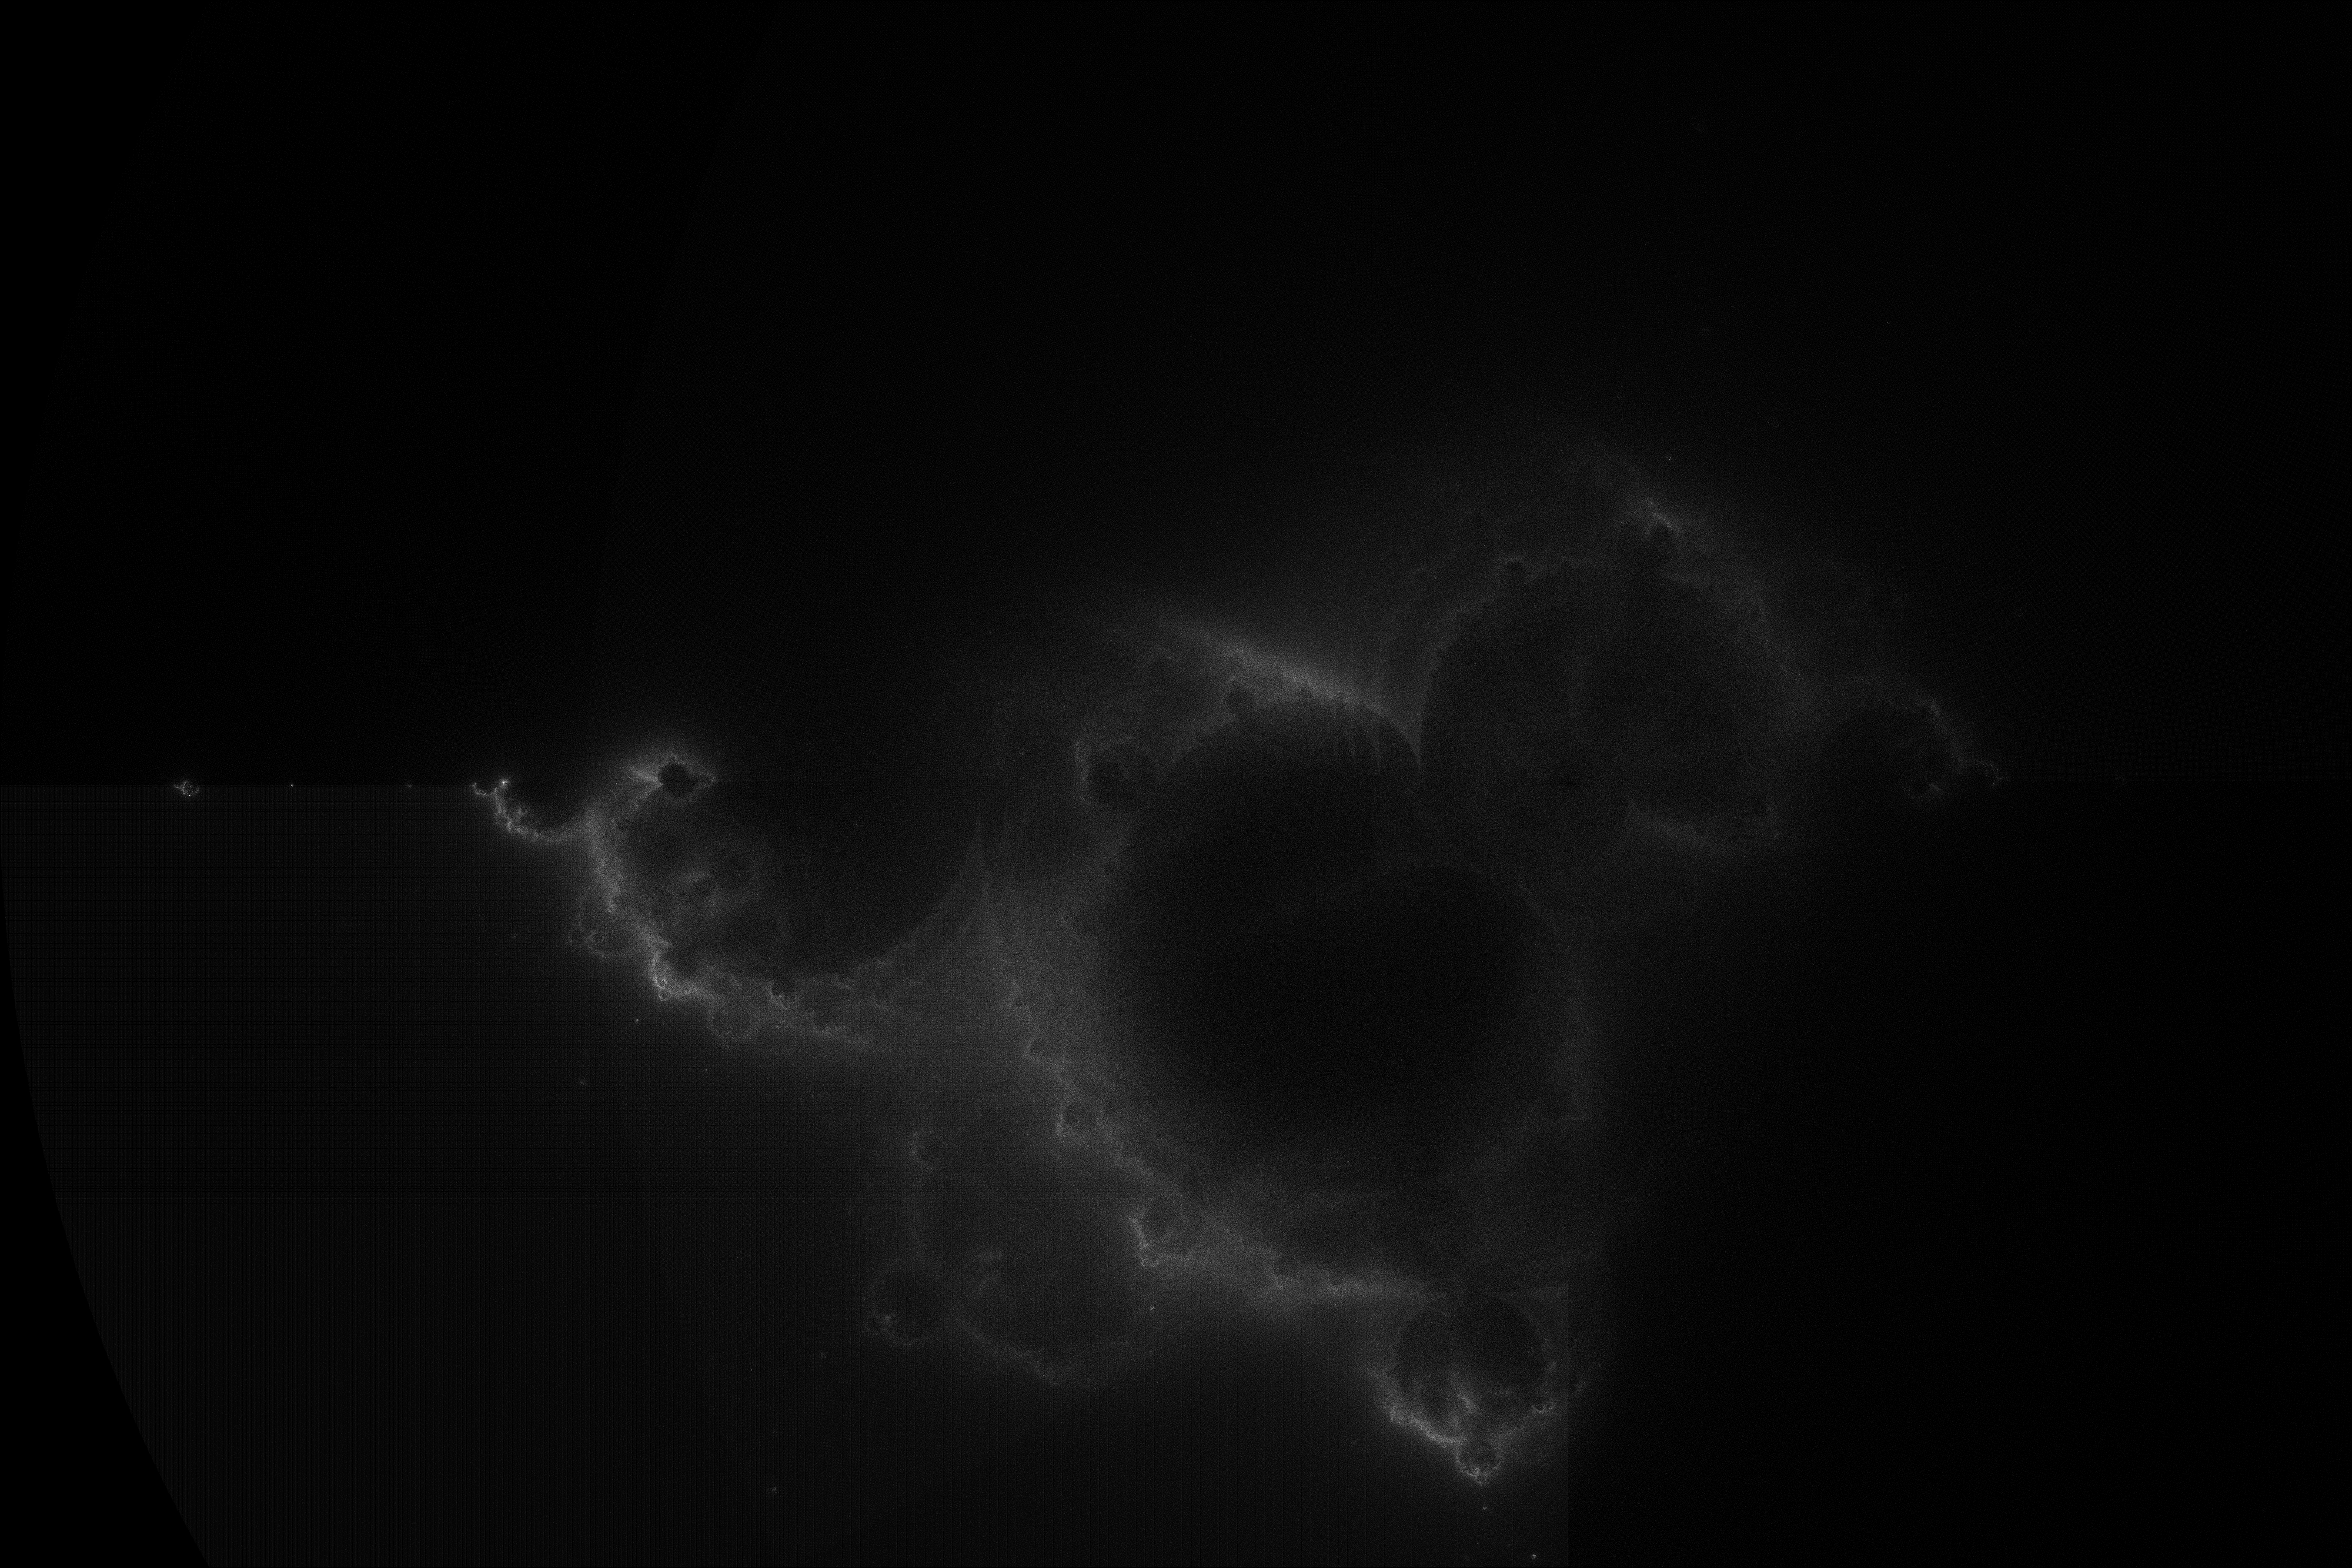
\includegraphics[width=.49\textwidth]{Pictures/2AnalyBuddhabrotmengeWithZoomGPU1ToPoint-0.5 + 0.0imWithIteration1000withResolution4000x2667.png}}\label{fig:2. Quadrant}}
	\hfill
	\subfloat[3. Quadrant]{\scalebox{1}[-1]{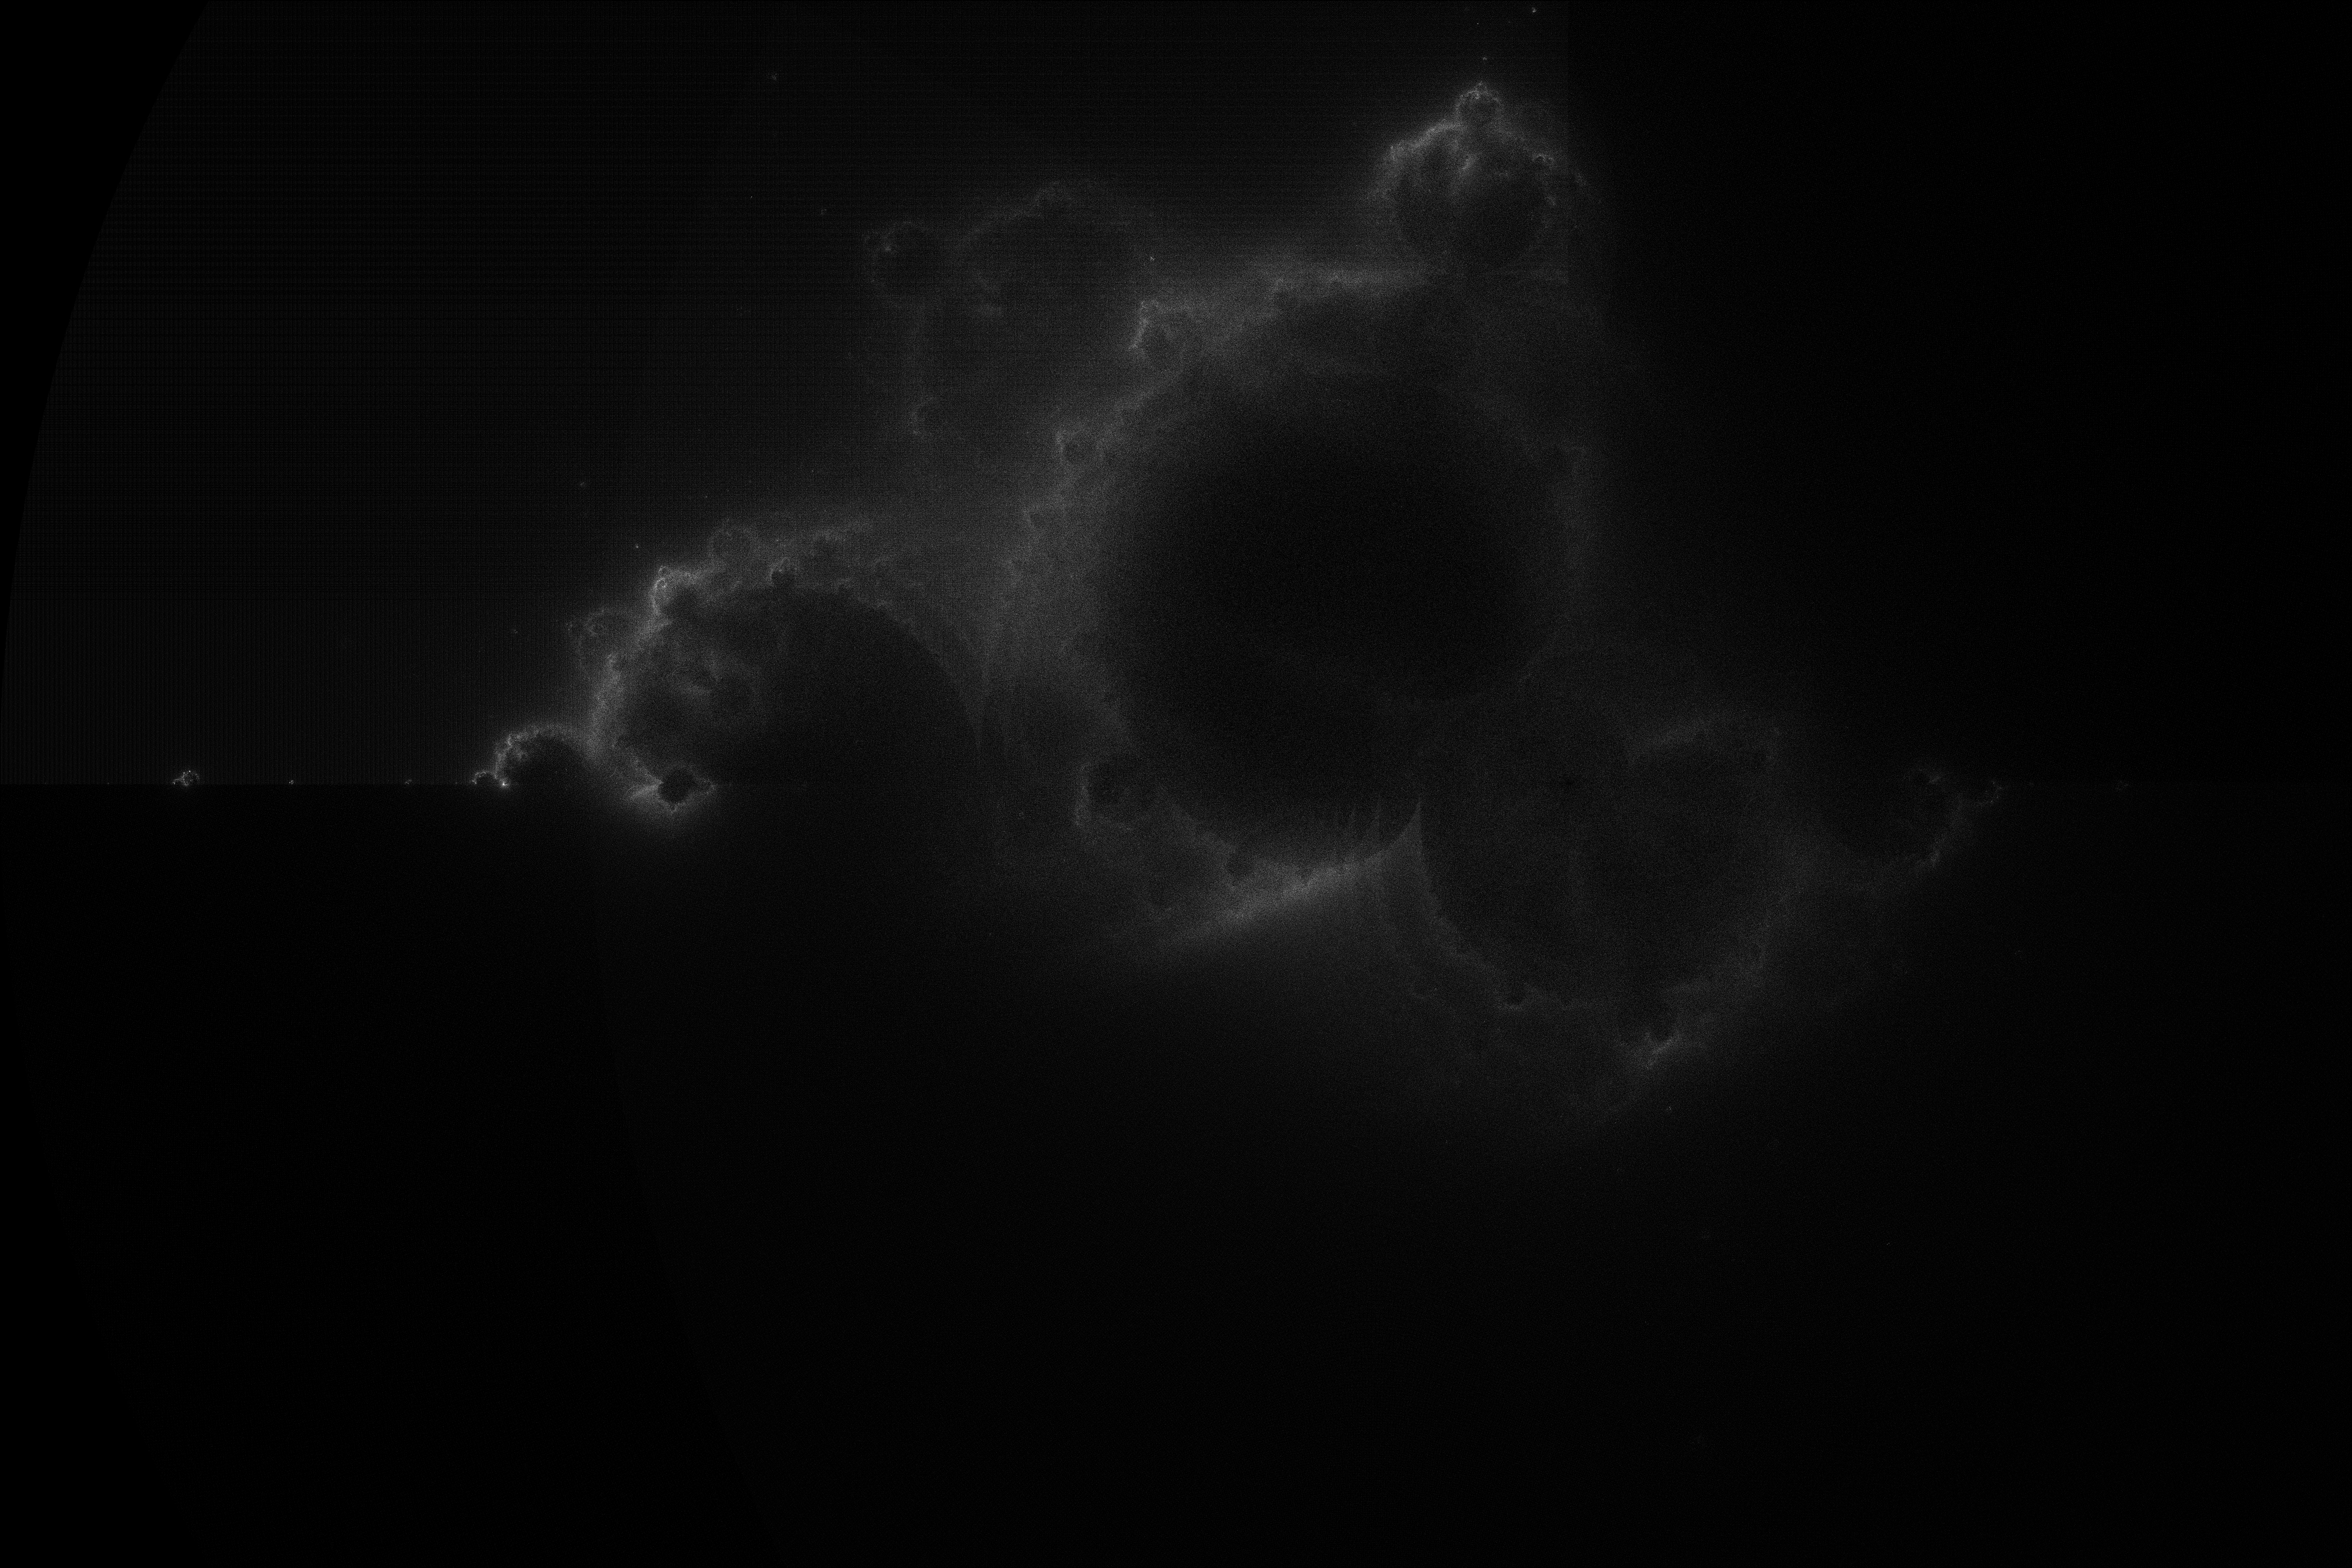
\includegraphics[width=.49\textwidth]{Pictures/3AnalyBuddhabrotmengeWithZoomGPU1ToPoint-0.5 + 0.0imWithIteration1000withResolution4000x2667.png}}\label{fig:3. Quadrant}}
	\hfill
	\subfloat[4. Quadrant]{\scalebox{1}[-1]{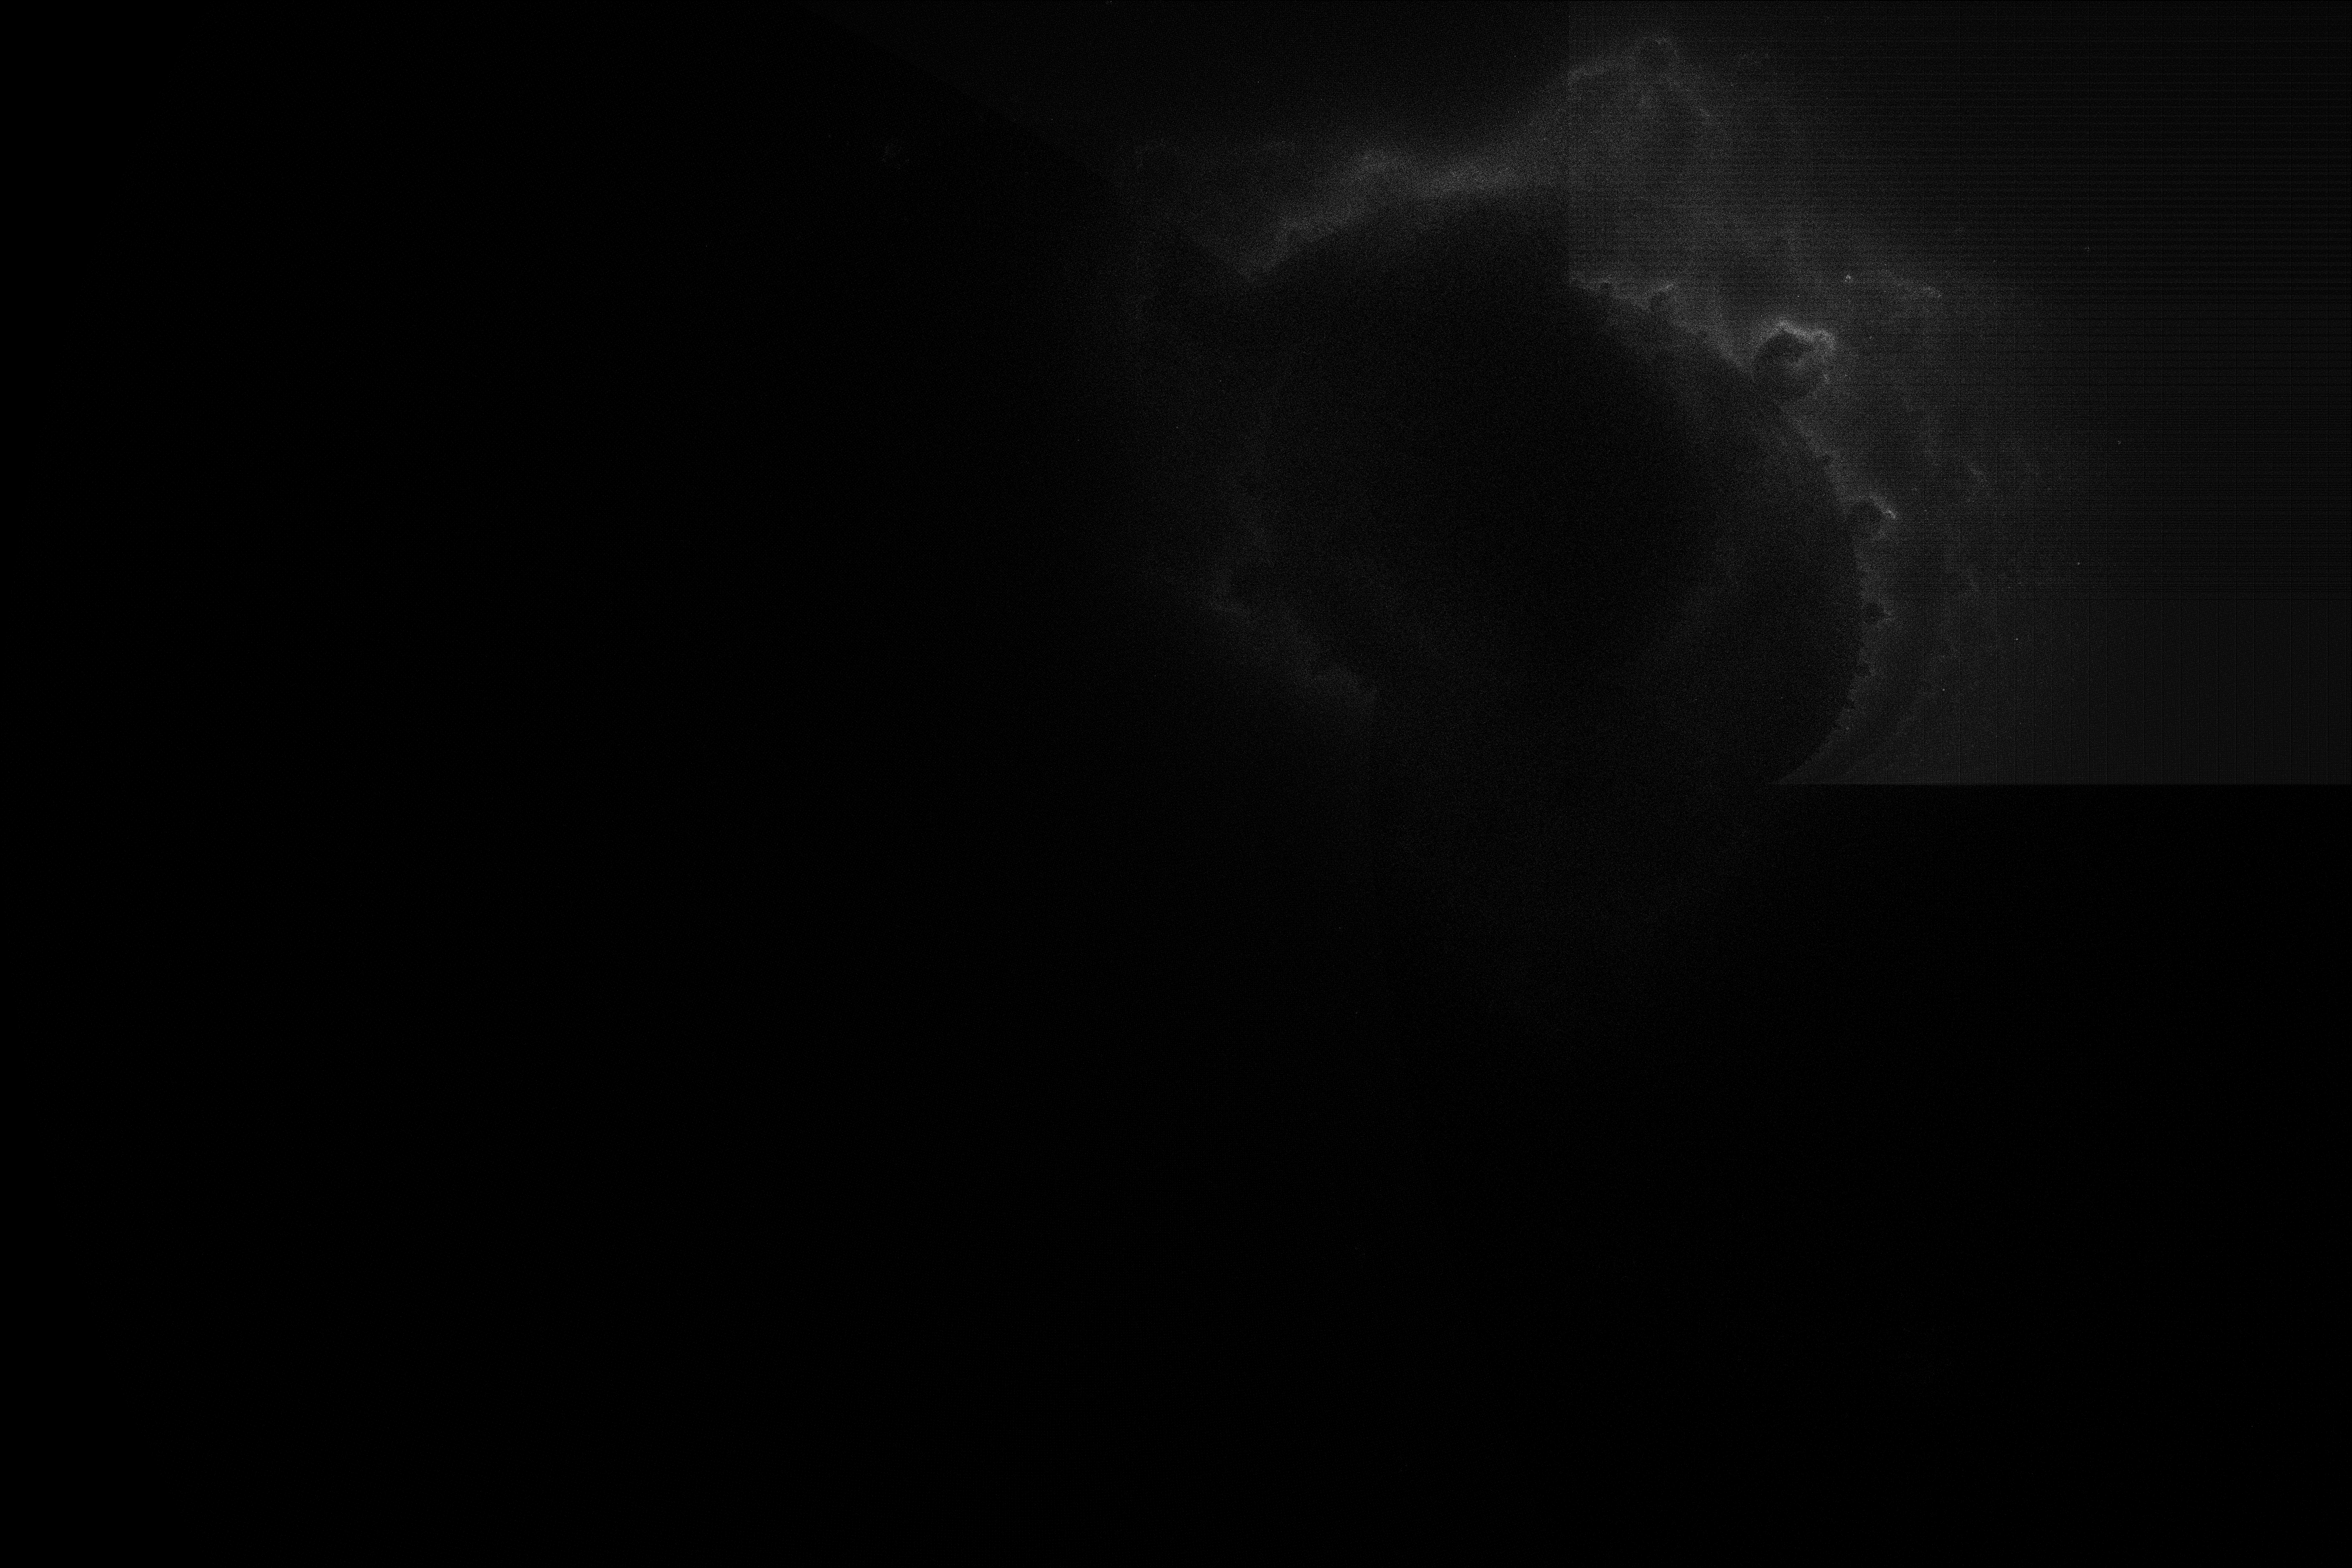
\includegraphics[width=.49\textwidth]{Pictures/4AnalyBuddhabrotmengeWithZoomGPU1ToPoint-0.5 + 0.0imWithIteration1000withResolution4000x2667.png}}\label{fig:4. Quadrant}}
\caption{Das Buddhabrot der einzelnen Quadranten}
\end{figure}
\begin{figure}[h!]
	\centering
	\subfloat[1. Quadrant]{\scalebox{1}[-1]{\includegraphics[width=.49\textwidth]{Pictures/10AnalyBuddhabrotmengeWithZoomGPU1ToPoint-0.5 + 0.0imWithIteration10000withResolution4000x2667.png}}\label{fig:1. Quadrant, abs}}
	\hfill
	\subfloat[4. Quadrant]{\scalebox{1}[-1]{\includegraphics[width=.49\textwidth]{Pictures/40AnalyBuddhabrotmengeWithZoomGPU1ToPoint-0.5 + 0.0imWithIteration10000withResolution4000x2667.png}}\label{fig:4. Quadrant, abs}}
	\caption{Das Buddhabrot für $\{z \in \mathbb{C}| |z|>1\}$ in den Quadranten 1 \& 4}
	\label{fig:absolute}
\end{figure}
Bei Abbildung \ref{fig:absolute} ist der auf einem Pixel maximal erreichte Wert vier.

\subsection{Implementierungszahlen}
Durch die gefundene Lösung ist ein 6.48-facher Zoom möglich. Bei einem, wie zuvor erreichten Zoom von 6.25, braucht es nun mehr Zeit. Dies liegt daran, dass nun grosse Matrizen in einer Liste zu finden sind und so der Aufruf durch mehrere if-Konditionen länger dauert. Dies stellt jedoch einen lediglich geringen Verlust an Effizienz dar und ist somit irrelevant. Ein 6.48-facher Zoom zum Punkt -1.25 mit der Auflösung 4’002 auf 2’668 Pixel und mit 150 Iterationen dauert 3 Minuten und 53 Sekunden. Bei einem 6.25-fachem Zoom benötigt man bei dieser Lösung 3 Minuten und 41 Sekunde.
